\section{Reference Representation with a Coinductive Family}\label{sect:original}

Dually to the representation of finite triangles discussed in the
introduction, ``triangular matrices'' are now introduced as
\emph{infinite} square matrices, where the part below the diagonal has
been cut off. Recall that a type $E$ of elements outside the diagonal
is fixed throughout. If $A$ is the type of diagonal elements, then
$\Tri\,A$ shall denote the type of infinite triangular matrices with
$A$'s on the diagonal and $E$'s outside. The different $\Tri\,A$ are
coinductive datatypes that are all defined simultaneously, as was the
case for \Trif{}, hence they are a ``coinductive family of types'' or
``\emph{nested codatatype}'', as will be developed below.

\subsection{Infinite triangles as nested coinductive type}

Infinite triangles can also be visualized as in \rfig{visu_col}, this time with the dots representing an infinite extension.



If we now cut the triangle into the first column and the rest, we get one
element of $A$ (as before for \Trif{}) and a trapezium, with an uppermost row
consisting of infinitely many $E$'s.

The $n$-th column consists of an element of $A$ on the diagonal and
$n$ elements of $E$ above the diagonal, as in the case of \Trif{}. As
before, we do not want to parameterize the type of the columns by
their index and instead integrate the side diagonal into the diagonal --
and this has to be done corecursively \cite{grossestcspaper}.
This integration is possible since trapeziums are again in one-to-one
correspondence to triangles, as shown in \rfig{tri_trap}, now interpreted infinitely.
In this figure, the trapezium to the left is considered as the
``trapezium view'' of the triangle to the right. Vice versa, the
triangle to the right is the ``triangle view'' of the trapezium to the
left.


We now formalize triangles through the following constructor that has to be interpreted coinductively.
\begin{definition}[$\Tri$, defined coinductively]\ 
    \begin{prooftree}
      \AxiomC {$a : A$}
      \AxiomC {$t : \Tri(E\times A)$}
      \doubleLine
      \BinaryInfC{$\constr\,a\,t : \Tri\,A$}
    \end{prooftree}
with $A$ a type variable.
\end{definition}


This means that the types $\Tri\,A$ for all types $A$ are simultaneously conceived as greatest solution to the fixed-point equation
$$Tri\,A = A \times \Tri(E\times A),$$
and \constr{} has two arguments instead of a pair of type $A\times\Tri(E\times A)$ just for technical convenience.

The second argument to \constr{} corresponds to the triangle view of the trapezium in our visualization in \rfig{visu_col}, but there
is no passage between a trapezium and a triangle -- this is only the motivation. In the formalization, there are only infinite triangles, but 
we set $\Trap\,A:=\Tri(E\times A)$ to hint to the trapezium view of these triangles.
\begin{definition}[Projections]\ 
  $$
  \begin{array}{l@{\hspace{2em}}l}
    \topT : \forall A.\,\Tri\,A \to A &
    \rest: \forall A.\, \Tri\,A \to \Trap\,A \\
    \topT\,(\constr\, a\, r) := a&
    \rest\,(\constr\, a\, r) := r
  \end{array}
  $$
\end{definition}
This definition by pattern matching implicitly uses the direction from
right to left in the above fixed-point equation. Thus, the top element and the trapezium part
of a triangle are calculated by unfolding the fixed point.

In order to obtain the triangle
that arises by cutting off the top row of a trapezium, we have to go
through all the columns.

\begin{definition}[$\cut:\forall A.\Trap\,A\to\Tri\,A$, defined corecursively]
$$\cut\,(\constr \,\pair e a\, r):=\constr\, a\,(\cut\, r)$$
\end{definition}

The definition does pattern matching on elements of $\Trap\,A$ and
constructs an element of the coinductive type $\Tri\,A$. The subterm
$\cut \,r$ represents a corecursive call to $\cut$, which is accepted
also by the Coq system as admissible corecursion since it is placed directly
as an argument to the constructor $\constr$.

\subsection{Redecoration for infinite triangles}

We are heading for a corecursive definition of the generic redecoration operation \redec{}
on triangles. It has type 
$$\forall A\forall B.\, (\Tri\,A\to B)\to\Tri\,A\to \Tri\,B,$$
which is the type of a coextension operation for $\Tri$ viewed as
support of a comonad.  Coextension -- also called cobind -- is the
dual of the extension / bind operation of a monad, which is so
successfully used in the functional programming language Haskell.
The counit for the comonad we are about to construct is our \topT{} operation.

Redecoration for \Tri{} follows the same pattern as for \Trif{}, but the successive applications of the same operation will never reach a base case, as there is none in \Tri{}. 


Formally, this is done by a corecursive definition, where
$\redec\,f\,t$ for $t$ of type $\Tri\,A$ has to call itself with
second argument of type $\Trap\,A$, hence $f$ is not even type-correct
as a first argument in that corecursive call. Instead of $f:\Tri\,A\to
B$, a ``lifted'' version of $f$ is needed that has type $\Tri(E\times
A)\to E\times B$.
\begin{definition}[$\lift:\forall A\forall B.\,(\Tri\,A\to B)\to \Tri(E\times A)\to E\times B$]
$$\lift\,f\,r:=\pair{\fst(\topT\,r)}{f(\cut\,r)}\enspace,$$
where $\fst$ is the first projection (from a pair to its first
component).  
\end{definition}
The definition is illustrated in \rfig{lift}.
\begin{figure}[h]
  \centering
  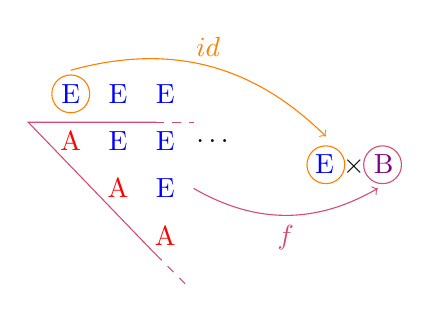
\begin{tikzpicture}[scale = 0.6]
    \foreach \y in {0,...,2}
    {\foreach \x in {\y,...,2}
      \draw (\x+1, -\y) node[color=blue]{E} ;
    }
    \foreach \x in {1,...,3} \draw (\x, -\x) node[color=red]{A} ;
    \draw(4,-1) node{$\ldots$};

     \draw (7,-1.5) node{{\color{blue} E} $\times$ {\color{violet} B}} ;
    \draw[color=orange] (1,0) circle(0.4cm);
    \draw[color=orange] (6.4,-1.5) circle(0.4cm);
    \draw[color=purple!70]  (2.8, -3.4) --
     (0.1,-0.6) -- (2.8,-0.6);
    \draw[color=purple!70, dashed]  (2.8,-0.6) -- (3.6,-0.6);
    \draw[color=purple!70, dashed]  (2.8,-3.4) -- (3.5,-4.1);

    \draw[color=purple!70] (7.6,-1.5) circle(0.4cm);

     \draw[->, color = orange] (1,0.5) to [bend left] node[auto,
     swap, above]{$id$} (6.4,-0.9) ; 
    \draw[->, color = purple!70] (3.6,-2) to [bend right] node[auto,
    swap, below]{$f$} (7.5,-2) ; 
    
  \end{tikzpicture}
  \vspace{-3ex}
  \caption{Definition of lifting}
  \label{fig:lift}
\end{figure}

The formal definition of redecoration is as follows:
\begin{definition}[$\redec:\forall A\forall B.\,(\Tri\,A\to B)\to \Tri\,A\to\Tri\,B$, defined corecursively]
$$\redec\,f\,t:=\constr\, (f\,t)\,\bigl(\redec\,(\lift\,f)\, (\rest\,t)\bigr)\enspace,$$
\end{definition}
see \rfig{redec}. 
This definition is accepted since it is guarded: the corecursive
call to $\redec$ is as second argument to $\constr$, and it does not
matter that the argument $f$ becomes $\lift\,f$ there. A function
argument that becomes more complicated in the recursive call is
typical of recursion on nested datatypes, see, e.\,g.,
\cite{grossestcspaper}.
\begin{figure}[h]
  \centering
  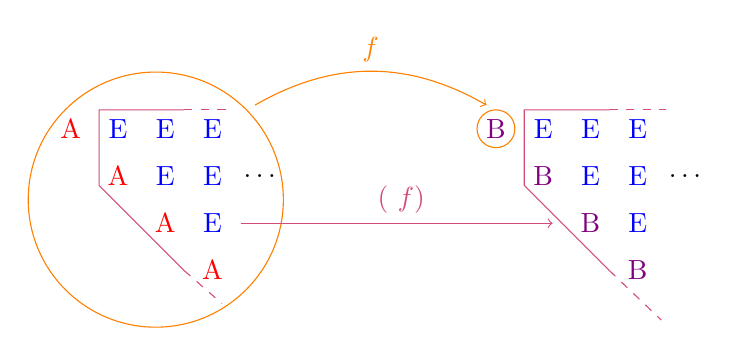
\begin{tikzpicture}[scale = 0.6]
    
    \foreach \y in {0,...,2}
    {\foreach \x in {\y,...,2}
      \draw (\x+1, -\y) node[color=blue]{E} ;
    }
    \foreach \x in {0,...,3} \draw (\x, -\x) node[color=red]{A} ;
    \draw(4,-1) node{$\ldots$};

    \foreach \y in {0,...,2}
    {\foreach \x in {\y,...,2}
      \draw (\x+10, -\y) node[color=blue]{E} ;
    }
    \foreach \x in {0,...,3} \draw (\x+9, -\x) node[color=violet]{B} ;
    \draw(13,-1) node{$\ldots$};
    \draw[color=purple!70]  (2.4, -3) --
    (0.6,-1.2) -- (0.6,0.4) -- (2.4,0.4);
    \draw[color=purple!70, dashed]  (2.4,0.4) -- (3.4,0.4);
    \draw[color=purple!70, dashed]  (2.4,-3) -- (3.2,-3.7);
 
    \draw[color=orange] (1.8,-1.5) circle(2.7cm);

    \draw[color=purple!70]  (11.4, -3) --
    (9.6,-1.2) -- (9.6,0.4) -- (11.4,0.4);
    \draw[color=purple!70, dashed]  (11.4,0.4) -- (12.6,0.4);
    \draw[color=purple!70, dashed]  (11.4,-3) -- (12.5,-4.05);
    
    \draw[color=orange] (9,0) circle(0.4cm);
    
    \draw[->,color = orange] (3.9,0.5) to [bend left] node[auto,
    swap, above]{$f$} (8.8,0.5) ; 

    \draw[->,color = purple!70] (3.6,-2) to node[auto,
    swap, above]{$\redec~(\lift~f)$} (10.2,-2) ; 
    
  \end{tikzpicture}
  \caption{Definition of redecoration}
  \label{fig:redec}
\end{figure}

This completes the definition, but leaves open the question if this is
really (in what sense) the cobind of a comonad and if it corresponds
to operations that are easier to understand than corecursion on nested
codatatypes. We note that recursion schemes for nested datatypes have
been subject of a long line of research, starting from work by Bird
and colleagues
\cite{birdmeertens,gfolds}.


\subsection{Properties of redecoration}

It is well-known that propositional equality $=$ (called Leibniz
equality in Coq since $t_1=t_2$ allows the replacement of $t_1$ by
$t_2$ in any mathematical context) cannot suffice as criterion for the
correctness of elements that are calculated in coinductive
types. Propositional equality cannot be established by coinductive
reasoning because this is confined to coinductively defined
conclusions, and propositional equality is not coinductive (in Coq, it
is defined inductively).  We write $\Rel\,C$ for the type of the
binary relations on $C$, and we use these relations in infix
notation. In Coq, their type is $C\to C\to\Prop$, where $\Prop$ is the
universe of propositions.

\begin{definition}[$\bisim:\forall A.\,\Rel(\Tri\,A)$, defined
  coinductively]\ 
        \begin{prooftree}
          \AxiomC {$t_1\,,\, t_2 : \Tri\,A$}
          \AxiomC {$\topT\,t_1 = \topT\,t_2$}
          \AxiomC {$\rest\,t_1\bisim\rest\,t_2$}
          \doubleLine
          \TrinaryInfC{$t_1\,\bisim\, t_2$}
        \end{prooftree}
\end{definition}
It is easy to show that \bisim{} is an equivalence relation for any
argument type $A$. It is an equivalence relation but not a congruence:
for every operation of interest we have to establish compatibility
with bisimilarity. This is in particular easily done for the
projection functions \topT{} and \rest{} and for the \cut{} operation.

Using this notion of bisimilarity, we can show that \redec{} is
extensional in its function argument (modulo \bisim{}), using full
extensionality of \lift{}:
\begin{lemma}\label{lemma:liftext}
  $\forall A \forall B \forall (f\, f': \Tri\,A \to B).\, 
  (\forall t, f\,t = f'\, t) \Rightarrow \forall t, \lift\,f\,t = \lift\,f'\, t$
\end{lemma}
\begin{lemma}
  $\forall A \forall B \forall (f\, f': \Tri\,A \to B).\, 
  (\forall t, f\,t = f'\, t) \Rightarrow \forall t, \redec\,f\,t \bisim \redec\,f'\, t$
\end{lemma}

The main properties of \redec{} we are interested in express that
\topT{} and \redec{} together constitute a comonad for ``functor''
\Tri{}.  The precise categorical definition in coextension form (with
a cobind operation instead of the traditional comultiplication) is,
e.\,g., given in \cite{DBLP:conf/sfp/UustaluV01}. Here, we give the
constructive notion we use in this paper, and it is parameterized by
an equivalence relation while classically, only mathematical equality
$=$ is employed.

\begin{definition}[Constructive comonad]
  A constructive comonad consists of a type transformation $T$, a
  function $\counit:\forall A.\,T\,A\to A$, a function
  $\cobind:\forall A\forall B.(T\,A\to B)\to T\,A\to T\,B$ and an
  equivalence relation $\simcom:\forall A.\,\Rel(T\,A)$ such that the
  following comonad laws hold:
\begin{eqnarray}
&&\forall A\forall B\forall f^{T\,A\to B}\forall t^{T\,A}.\, \counit (\cobind\,f\,t) = f\,t \\
&&\forall A\forall t^{T\,A}.\,\cobind\,\counit_A\,t \simcom t \\
&&\forall A\forall B\forall f^{T\, A \to B}\forall g^{T\, B \to C}\forall t^{T\, A}.\,\cobind\,(g \circ \cobind\,f)\,t \simcom\cobind\,g\,(\cobind\,f\,t)\label{thirdlaw}
  \end{eqnarray}
\end{definition}
Here, in order to save space, we gave the type information for the
term variables as superscripts. The index $A$ to \counit{} is meant to
say that the type parameter to \counit{} is set to $A$ -- in all other
cases, we leave type instantiation implicit.

\begin{definition}[Constructive weak comonad]
  A constructive weak comonad is defined as a constructive comonad,
  but where the equation in (\ref{thirdlaw}) is restricted to
  functions $g$ that are compatible with $\simcom$ in the following
  sense: $\forall t\,t', t \simcom t' \Rightarrow g\,t = g\,t'$.
\end{definition}

\begin{lemma}\label{lemma:TriWComonad}
  The type transformation \Tri{}, the projection function \topT{} and
  \redec{} form a constructive weak comonad with respect to \bisim{}.
\end{lemma}

The first comonad law is satisfied in an especially strong form:
$\topT(\redec\,f\,t)$ actually \emph{is} $f\,t$ by definition.  The
other comonad laws go through with suitable generalizations of the
lemmas -- in order to ensure guardedess of the proofs. The current
solution is unspectacular, but it was not obvious how to do it (much
more complicated solutions were found on the way and are now
obsolete). We only show the strengthening of the second comonad law,
but it is the same style for the third one.
\begin{lemma}[strengthened form of second comonad law for $\redec$]
  $$\forall A\forall (f:\Tri\,A\to A).\,(\forall (t:\Tri\,A), f\,t = \topT\,t) \Rightarrow \forall (t:\Tri\,A).\,\redec\,f\,t\bisim t$$
\end{lemma}
The proof is by coinduction and uses \rlem{liftext}. Obviously, this
implies the second comonad law.  For all the details, see our
formalization in Coq
\cite{TYPES11code}. We only get a weak comonad because proving
pointwise equality of $\lift (g \circ (\redec\,f))$ and $(\lift\, g)
\circ (\redec (\lift\,f))$ requires compatibility of $g$ with
\bisim{}, and this is a crucial step for proving the third comonad
law.

\medskip
When defining the \cut{} operation, one might naturally want to get also
the part that has been cut out (the elements of $E$). 
These elements are given by the following function:
\begin{definition}[$\escut : \forall A.\, \Trap\,A \to \Str\,E$, defined corecursively]
  $$\escut\,(\constr\,\pair e a\, r) := e :: (\escut\,r)$$
\end{definition}
\begin{remark}
  In the standard library of Coq, the type of streams with elements in type $C$ are predefined, and we can represent this definition as follows:
  \begin{prooftree}
    \AxiomC {$c : C$}
    \AxiomC {$s: \Str\,C$}
    \doubleLine
    \BinaryInfC{$c :: s : \Str\,C$}
  \end{prooftree}
  The projection functions are called \hd{} and \tl{}. They are such
  that $\hd(c :: s) = c$ and $\tl(c :: s) = s$. 
  We will also use the \map{} function defined by $\map\,f\,(c :: s) =
  f\,c :: (\map\,f\,s)$.
  
\end{remark}
Using \escut{}, we can define the first row of $E$ elements in a triangle as
$$\frow:\forall A.\,\Tri\,A\to\Str\,E\qquad\qquad\frow\,t:=\escut\,(\rest\,t)$$


Once we have these definitions, we might want to be able to ``glue''
the two cut parts in order to recreate the original trapezium. This is
done by the function \addes{}
\begin{definition}[$\addes : \forall A.\, \Str\,E \to \Tri\,A \to
  \Trap\, A$, defined corecursively]
  $$\addes\,(e :: \es)\,(\constr\, a\, r) := \constr\,\pair{e}{a}\,(\addes\,\es\,r)$$
\end{definition}
And it is then easy to show that \addes{} indeed performs the gluing:
$$ \forall A\forall(r:\Trap\,A).\, \addes\,(\escut\,r)\,(\cut\,r) \bisim r$$

%%% Local Variables:
%%% mode: latex
%%% TeX-master: "coredec"
%%% End:
